\documentclass[12pt]{article}

\usepackage{pablo-devoir}
\usepackage{pablo-listings}
\usepackage[a5paper,margin=1cm]{geometry}

\pagestyle{empty}

\title{Fonctions --- bis}
\date{2/12/14}
\classe{2\up{des}14}
\dsnum{DS 3}

\begin{document}

\maketitle

\begin{exercice}[Images et antécédents --- 7 points]
  \emph{Répondre aux questions par lecture graphique.}
  \begin{enumerate}
    \item On considère la fonction $f$ représentée ci-dessous.
  \begin{center}
    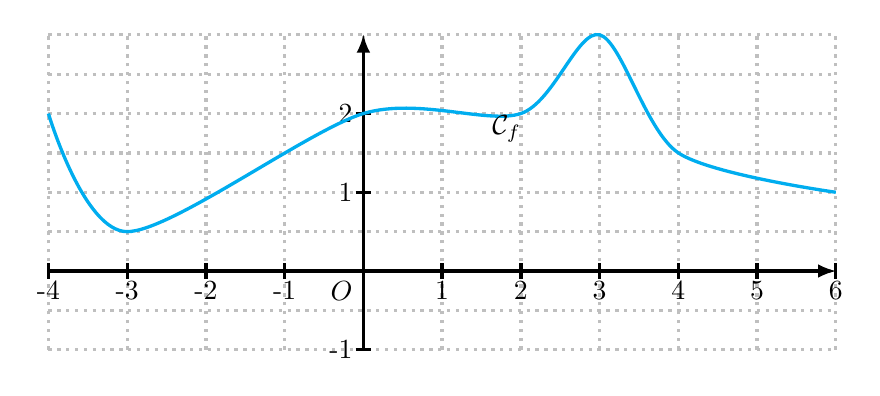
\begin{tikzpicture}[very thick,xscale=1, yscale=1]
      \draw[dotted, lightgray, xstep=1, ystep=.5] (-4, -1) grid (6, 3);
      \draw[-latex] (-4,0) -- (6,0);
      \draw[-latex] (0,-1) -- (0,3);
      \foreach \x in {-4, -3, -2, -1, 1, 2, 3, 4, 5, 6} {
        \draw (\x,0) node[below]{\x};
        \draw (\x,{0.1}) -- (\x,{-0.1});
      }
      \foreach \y in {-1, 1, 2} {
        \draw (0,\y) node[left]{\y};
        \draw (-.1, \y) -- (.1, \y);
      }
      \draw [cyan] plot [smooth, tension=0.5] coordinates {
        (-4,2)
        (-3, 0.5)
        (0, 2)
        (2, 2)
        (3, 3)
        (4, 1.5)
        (6, 1)
      };
      \draw (0,0) node[below left]{$O$};
      \draw (1.5, 1.5) node[above right]{$\mathcal{C}_f$};
    \end{tikzpicture}
  \end{center}
      \begin{enumerate}
        \item Déterminer $f(1)$.
        \item Déterminer l'image de $2$ par $f$.
        \item Quels sont le(s) antécédent(s) de $1$ par $f$ ?
        \item Résoudre graphiquement $f(x)=0$.
        \item Déterminer un nombre $k$ tel que $f(x)=k$ ait deux solutions.
      \end{enumerate}
    \item Déterminer les solutions de $g(x)=h(x)$ (où les courbes de $g$ et $h$ sont représentées ci-dessous).
      \begin{center}
        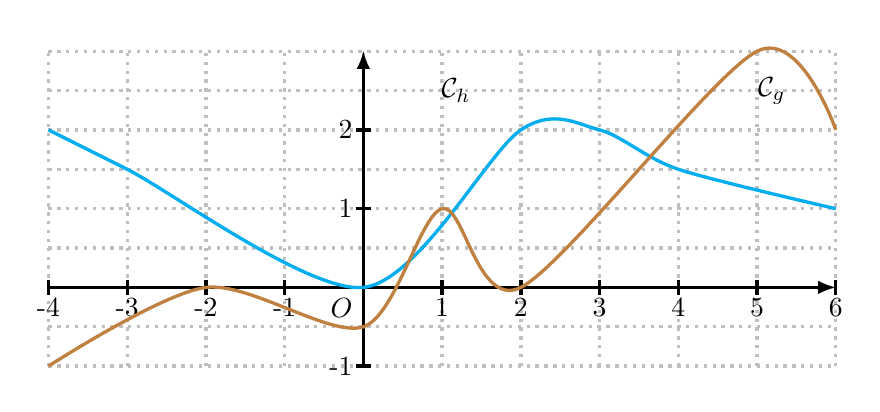
\begin{tikzpicture}[very thick,xscale=1, yscale=1]
          \draw[dotted, lightgray, xstep=1, ystep=.5] (-4, -1) grid (6, 3);
          \draw[-latex] (-4,0) -- (6,0);
          \draw[-latex] (0,-1) -- (0,3);
          \foreach \x in {-4, -3, -2, -1, 1, 2, 3, 4, 5, 6} {
            \draw (\x,0) node[below]{\x};
            \draw (\x,{0.1}) -- (\x,{-0.1});
          }
          \foreach \y in {-1, 1, 2} {
            \draw (0,\y) node[left]{\y};
            \draw (-.1, \y) -- (.1, \y);
          }
          \draw [cyan] plot [smooth, tension=0.5] coordinates {
            (-4,2)
            (-3, 1.5)
            (0, 0)
            (2, 2)
            (3, 2)
            (4, 1.5)
            (6, 1)
          };
          \draw [brown] plot [smooth, tension=0.5] coordinates {
            (-4,-1)
            (-2, 0)
            (0, -.5)
            (1, 1)
            (2, 0)
            (5, 3)
            (6, 2)
          };
          \draw (0,0) node[below left]{$O$};
          \draw (1.5, 2.5) node[left]{$\mathcal{C}_h$};
          \draw (5.5, 2.5) node[left]{$\mathcal{C}_g$};
        \end{tikzpicture}
      \end{center}
  \end{enumerate}

\end{exercice}

\pagebreak

\begin{exercice}[Variations --- 4 points]
  On considère une fonction $f$, définie sur $\left[ 0;10 \right]$, croissante sur $\left[ 0;6 \right]$ et décroissante ensuite.

      \begin{enumerate}
        \item Dresser le tableau de variations de $f$.
        \item Comparer $f(6)$ et $f(8)$.
      \end{enumerate}
\end{exercice}

\begin{exercice}[Algorithme --- 2 points]
  Un magasin de bricolage vend des vis au tarif suivant.
  \begin{itemize}[$\bullet$]
    \item Les cent premières vis : 0,01~\euro{} pièce ;
    \item Les quatre-cents suivantes : 0,005~\euro{} pièce ;
    \item Toutes les autres : 0,001~\euro{} pièce.
  \end{itemize}

  Recopier sur votre copie l'algorithme suivant, et le compléter, pour qu'étant donné un nombre $n$, il affiche le prix de $n$ vis.
      \begin{lstlisting}[language=naturel,frame=lines,mathescape=true]
      Lire n
      Si ...
      Alors
        Afficher 0,01 * n
      Sinon
        ...
      FinSi
      \end{lstlisting}
\end{exercice}

\begin{exercice}[Problème --- 7 points]
  Dans un grenier de forme triangulaire (voir shéma ci-dessous), on souhaite construire une chambre de la forme d'un pavé droit qui ait le volume le plus grand possible.

  Voici la coupe du grenier (triangulaire) et de la chambre (grisée).

  \begin{multicols}{2}
  \begin{center}
  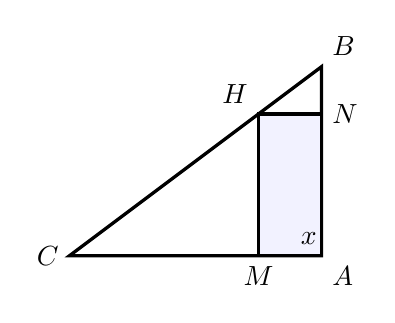
\begin{tikzpicture}[very thick,scale=.8]
    \draw (0,0) node[left]{$C$} -- ++(4,0) node[below right]{$A$} -- ++(0,3) node[above right]{$B$} -- cycle;
    \draw[fill=blue!5] (3,0) node[below]{$M$} -- (3,{9/4}) node[above left]{$H$}-- (4,{9/4}) node[right]{$N$} -- (4,0) -- cycle node[midway,above right]{$x$};
  \end{tikzpicture}
\end{center}

On nomme $x$ la longueur $AM$.

On donne (en mètres) $BA=3$ et $AC=4$.
\end{multicols}

\begin{enumerate}
  \item On appelle $\mathcal{A}(x)$ l'aire (en $m^2$) du rectangle $AMHN$.
\begin{enumerate}
  \item Quelles valeurs peut prendre $x$ ?
  \item Montrer que $HM=\frac{3}{4}\left( 4-x \right)$.
  \item En déduire que l'aire $\mathcal{A}(x)$ est $\frac{3}{4}x\left( 4-x \right)$.
\end{enumerate}
\item On a tracé les variations de $\mathcal{A}$ dans le tableau suivant.

  \begin{center}
        \begin{tikzpicture}[xscale=1,yscale=1]
          \tkzTabInit[lgt=1,espcl=2]
          {$x$ /1,
            $\mathcal{A}$ /2
          }
          {0, {2}, 4}%
          \tkzTabVar{-/0, +/{3}, -/0}
        \end{tikzpicture}
      \end{center}
      \begin{enumerate}
        \item Quelle est l'aire maximale que peut prendre le rectangle $AMHN$.
        \item Quelle est alors sa forme ?
      \end{enumerate}
\end{enumerate}
\end{exercice}

\end{document}
